\documentclass[a4paper]{article}
\usepackage{afterpage}
\usepackage{caption}
\usepackage{subcaption}
\usepackage{hanging}
\usepackage{setspace}
\usepackage[a4paper, margin=1.2in, footnotesep=1.5\baselineskip]{geometry}
\usepackage[
backend=biber,
style=chem-biochem,
citestyle=nature,
url=false,
doi=true,
isbn=false,
autocite=superscript
]{biblatex}
\usepackage{todonotes}
\usepackage{doi}
\usepackage{titlesec}
\usepackage{hyperref}
\usepackage{caption}
\usepackage{subcaption}
\usepackage{pdflscape}

\renewcommand{\thefootnote}{\alph{footnote}}
%\newcommand{\sectionbreak}{\clearpage}
\renewcommand*{\bibfont}{\footnotesize}
\addbibresource{../references.bib}
\bibliographystyle{unsrtnat}
\urlstyle{rm}

\hypersetup{
    colorlinks=true,
    citecolor=magenta,
    linkcolor=magenta
}

\setlength{\parskip}{0.75em}

\onehalfspacing

\pagestyle{plain}

\graphicspath{ {./figures/} }

\renewcommand{\abstractname}{Summary}

\title{
	{\normalsize Doctoral Confirmation Report} \\
	{\LARGE \textsc{Building Resilience: How do Species Interactions Shape Ecosystem Collapse?}}
}
\author{
  {\large Fernando Cagua}
}
\date{}

\begin{document}

\maketitle







\section*{Introduction}

The present report summarises the advances made since the presentation of the PhD proposal in August 2015. The literature review and the description of the research, including the planned methodology and analysis techniques has already been included in the PhD proposal and will not be expanded here (the PhD proposal is attached to this report). Here I focus on presenting the results obtained to date. To date there have not been changes on the scope or the research objectives, neither on the methodology or the proposed timeline.

Natural ecosystems provide important services---like food and water---we humans depend on to a large extent.
  Much like the failure of a single key financial institution can trigger unexpected crashes on the stock market, human pressures---such as biological invasions and species extinctions---can cause sudden collapses that severely transform the way ecosystems function.
  However, despite its importance, we do not completely understand the dynamics that make ecosystems resilient to collapse.
  Because the functioning of ecosystems is largely determined by the network of interactions between the species that inhabit them, my proposed research aims to quantify the role played by species interactions in determining the resilience of ecosystems.
  To achieve this, I will focus on networks of mutually beneficial interactions, like those between plants and their pollinators, and use a combination of empirical data, computer simulations and ecological theory.
  Ultimately I want to understand why, when and how ecosystem collapses occur, and how to recover from them.

\section*{PhD objectives}

The overall objective of my proposed research is to quantify the role played by species interactions in modulating ecosystem resilience. 
To do so, I will focus on the network of mutualistic interactions between plants and pollinators \autocite{Bascompte2006, Bascompte2007, Klein2007}.
These networks, which form the base of pollination systems, play a globally important role in the maintenance of biodiversity and crop production \autocite{Bascompte2007, Klein2007}.

I will focus on empirically informed theoretical approaches.
Throughout my thesis, I will use computer simulated communities to estimate the population dynamics of the species in the community, and then I will directly quantify stability properties from fluctuations in the species populations \autocite{Bastolla2009, Garcia-Algarra2013}.
I will develop these `synthetic` communities under a wide range of parameters to answer the specific questions I aim to answer in each chapter of my dissertation.

In the first chapter of my thesis I will concentrate on biotic invasions.
Specifically I have a twofold objective: first, I aim to determine which network characteristics shape the its resistance and resilience to invasions, and second to determine how biotic invasions reshape network resistance and resilience by affecting existing interactions in the community.

Remarkably, invaded pollination communities have been shown to have structures that support more species \autocite{Stouffer2014} and can be more robust than those of un-invaded communities \autocite{Albrecht2014}.
Indeed we know which structures can enhance biodiversity \autocite{Bastolla2009} and delay the onset of catastrophic collapses \autocite{Lever2014}, but there are still serious mismatches between theoretical predictions and empirical observations.
I argue that this can be at least partially explained by the interplay between the degree of redundancy among species in the network and the apparent facilitation and competition between species in a mutualistic network.
Therefore, the objective of my second chapter is to evaluate the effects that structural redundancy has on the stability of ecological networks.

The aim of my third chapter is to obtain useful lessons for ecosystem management from a direct analysis the network structure.
Ecosystems are complex, non-linear systems that are very difficult to control.
On the other hand, recent work in theoretical physics has highlighted that is indeed possible to regulate them using targeted interventions \autocite{Cornelius2013}.
I propose to build upon these findings to determine the optimal set of management actions---from both a theoretical and a feasibility perspective---that are required to modify an ecosystem state.






\section*{Progress}

As specified on the PhD proposal schedule, I have started by the third objective of my thesis. However a thorough literature review and a outline of the research methodology has already been completed for Objectives 1 and 2. This can be found in the attached Research Proposal document. 

\begin{itemize}
	\item Objective 3: Controlling ecosystems for resilience management
	\begin{itemize}
		\item Objective 3.1. Determine the set of driver species: I've analised previously published data, and obtained preliminary results. An initial draft of the paper is underway. 
		\item Objective 3.2. Determine which interventions on the driver species are necessary to guide the ecosystem to the desired state: Ecosystem models are being currently developed by Jenny Shang, an intern under the University of Canterbury Summer Reserach Scholarship Programme. Results for this component are expected by mid February.
	\end{itemize}
\end{itemize}

\subsubsection*{Objective 3: Controlling ecosystems for resilience management}
 
\subsubsubsection{Introduction}

Ecosystems are challenging to ``control'' because they are large, complex, inhomogeneous, and non-linear systems.
However, recent work from theoretical physics has highlighted the possibility of regulating ecological networks by using targeted interventions in just some key species \autocite{Isbell2013, Cornelius2013}.
These species are not necessarily the most or least abundant, or invasive, but rather those that can drive the entire ecosystem dynamics \autocite{Liu2011} .
By modifying the abundances of driver species, it is in theory possible to control the state of the ecosystem, and possibly push the ecosystem into a pre-disturbance state or at least a more desirable alternate state of ecosystem function. To achieve that, the first step is to determine the smallest possible set of driver species in which to apply conservation measures that modify their abundance \autocite{Liu2011, Isbell2013}.

\subsubsubsection{Introduction}


I will determine these species by using `maximally matching' on the network of interactions---an algorithm that is already commonly used to find minimum sets in diverse areas of graph theory, image processing, and computational chemistry \autocite{Hopcroft1973,Neumann2010}.

By applying this framework to six pairs of invaded and uninvaded pollination networks \autocite{Bartomeus2008} I will examine the utility of this approach in a real world scenario.
Specifically I will explore the characteristics that make species (such as the degree of generalisation or it's contribution to nestedness) more or less likely to function as a driver of ecosystem state, and whether these characteristics depend on the presence of an invasive species in the ecosystem.

\section*{Research Plan}



\subsubsection*{Schedule:}
%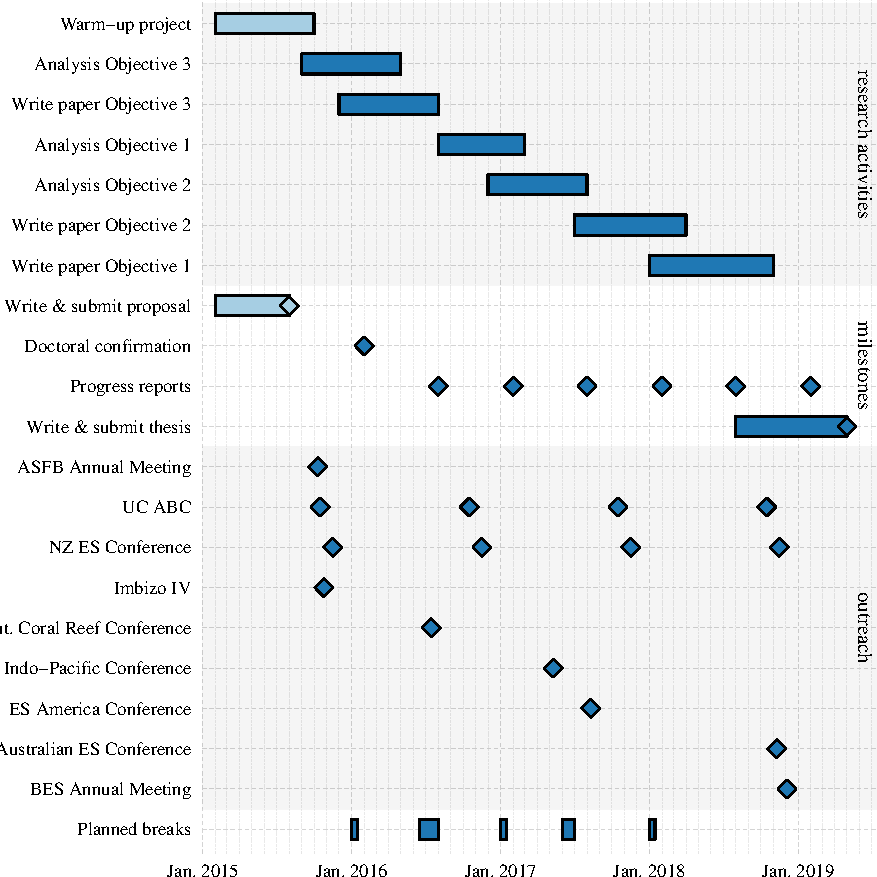
\includegraphics{schedule}
\end{landscape}

\printbibliography

\end{document}
